\documentclass[border=5mm]{standalone}
\usepackage{tikz}
\usepackage{amsmath}
\usetikzlibrary{shapes.geometric, arrows, positioning}

\begin{document}
	
    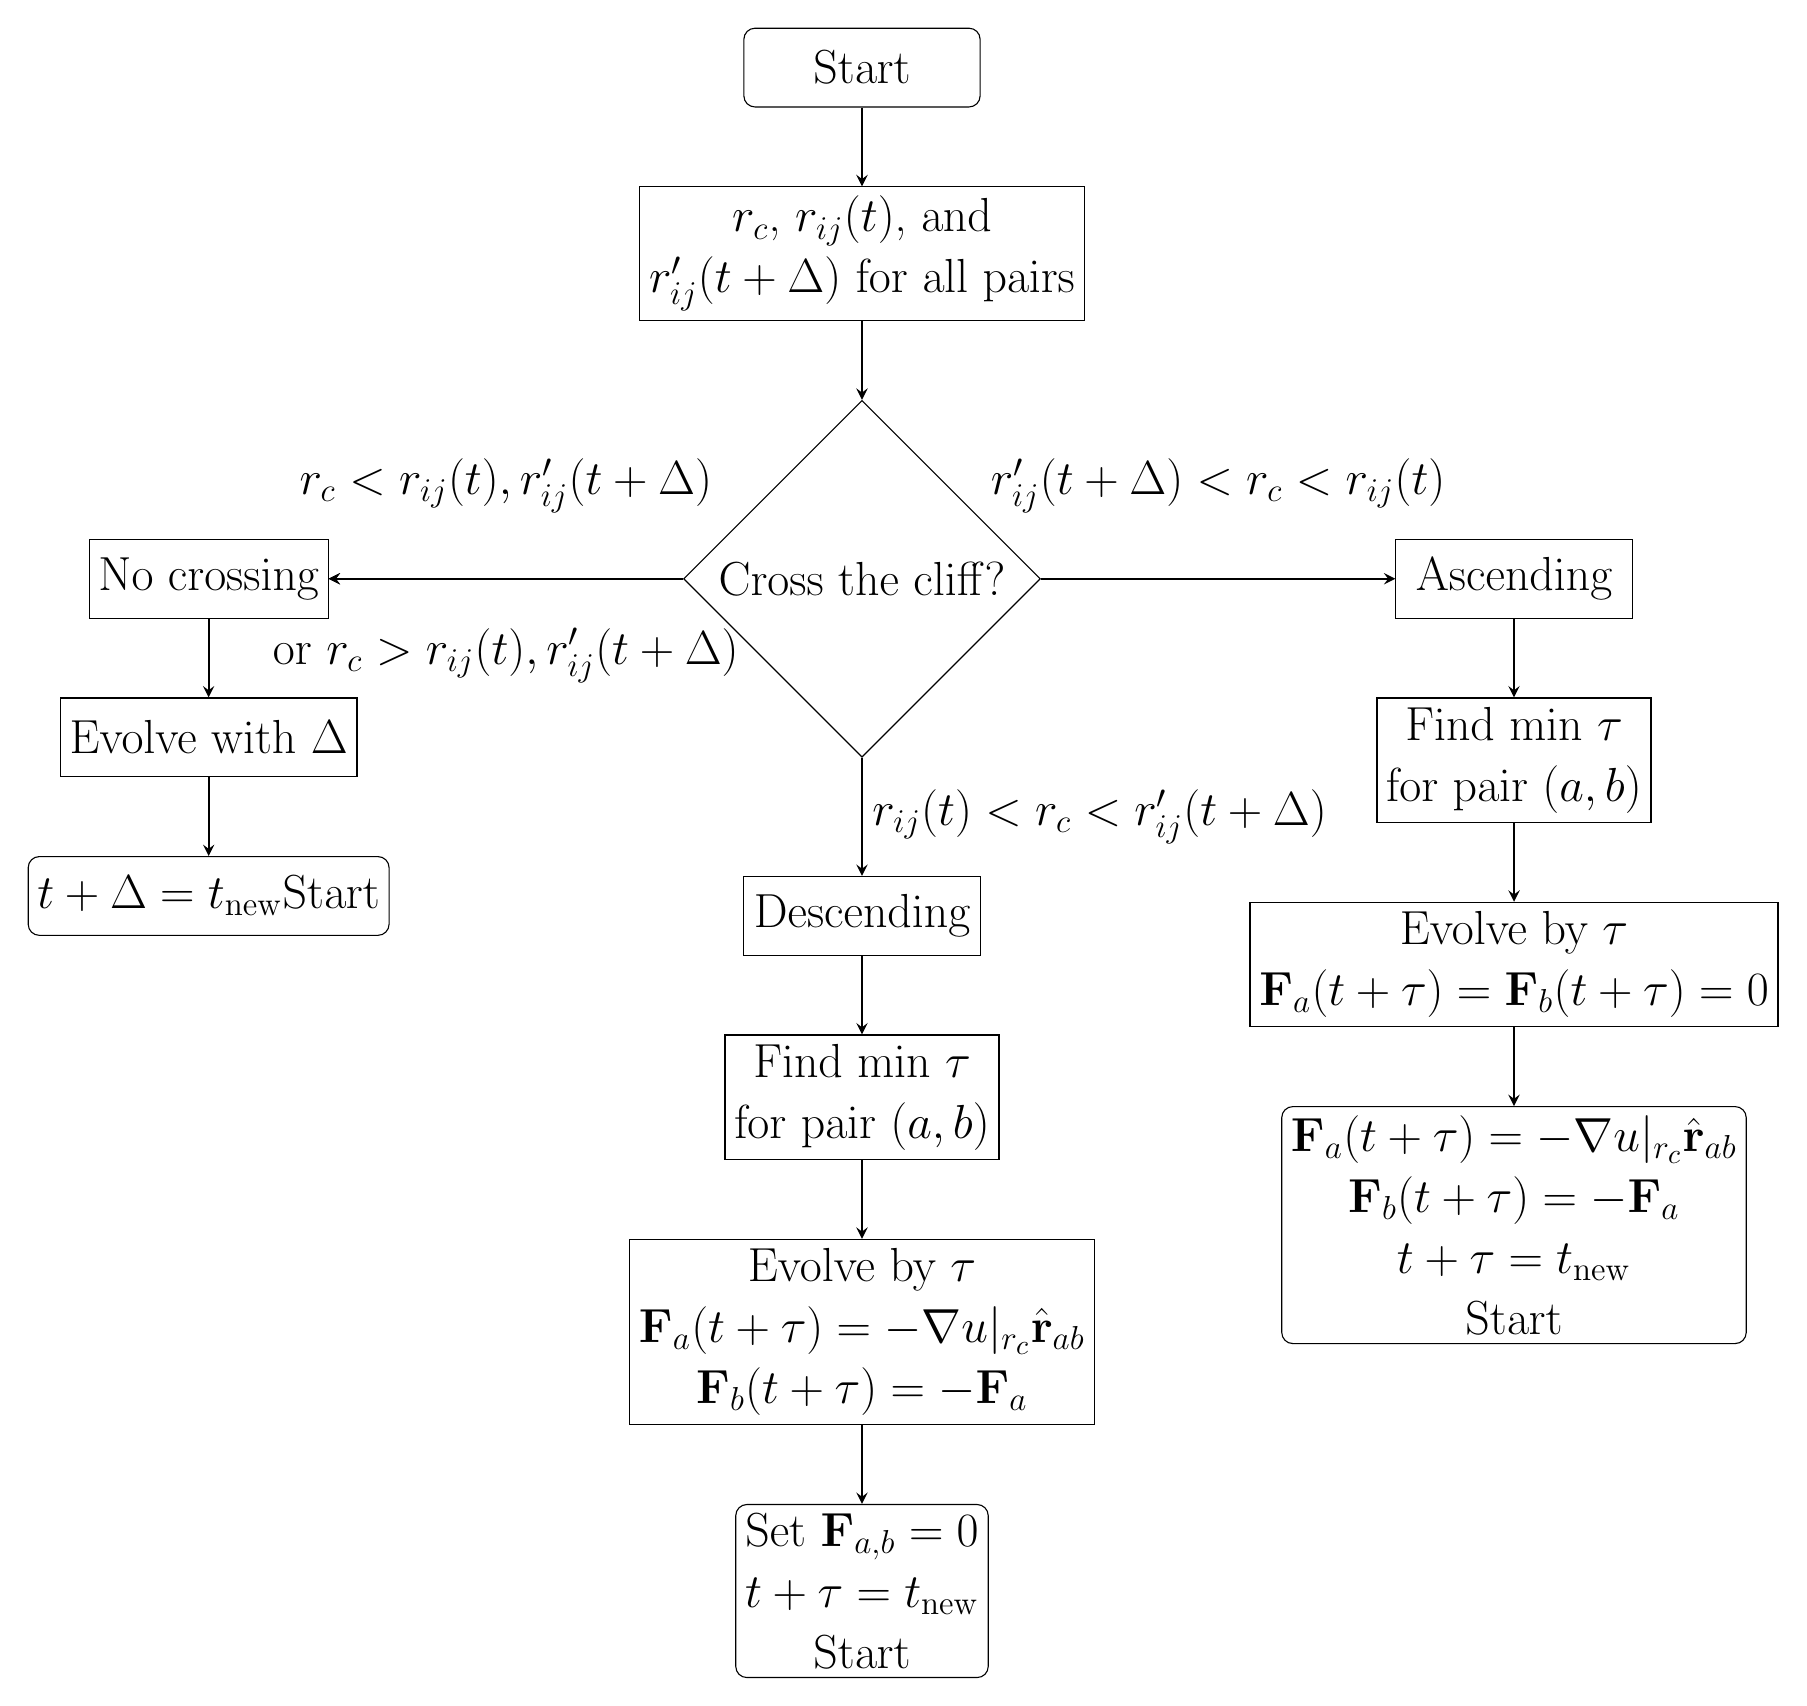
\begin{tikzpicture}[
    	startstop/.style={rectangle, rounded corners, minimum width=3cm, minimum height=1cm, text centered, draw=black, font=\LARGE},
    	process/.style={rectangle, minimum width=3cm, minimum height=1cm, text centered, draw=black, font=\LARGE},
    	decision/.style={diamond, minimum width=3cm, minimum height=1cm, text centered, draw=black, font=\LARGE},
    	arrow/.style={thick,->,>=stealth}
    	]
    	
    	% 中心判断节点
    	\node (check) [decision] {Cross the cliff?};
    	
    	% 开始和输入节点
    	\node (input) [process, above=of check, align=center] {$r_c$, $r_{ij}(t)$, and \\ $r_{ij}'(t+\Delta)$ for all pairs};
    	\node (start) [startstop, above=of input] {Start};
    	
    	% 左侧分支 - 否
    	\node (notcritical) [process, left=of check, xshift=-3.5cm, align=center] {No crossing};
    	\node (notcritical2) [process, below=of notcritical] {Evolve with $\Delta$};
    	\node (endnot) [startstop, below=of notcritical2] {$t+\Delta = t_{\mathrm{new}}$\\ Start};
    	
    	% 中间分支 - 下崖
    	\node (criticaldown) [process, below=of check, yshift=-0.5cm, align=center] {Descending};
    	\node (findmindown) [process, below=of criticaldown, align=center] {Find min $\tau$ \\ for pair $(a,b)$};
    	\node (evolvedown) [process, below=of findmindown, align=center] {Evolve by $\tau$ \\ $\mathbf{F}_a(t+\tau) = -\nabla u|_{r_c} \hat{\mathbf{r}}_{ab}$ \\ $\mathbf{F}_b(t+\tau) = -\mathbf{F}_a$};
    	\node (enddown) [startstop, below=of evolvedown, align=center] {Set $\mathbf{F}_{a,b}=0$ \\ $t+\tau = t_{\mathrm{new}}$ \\ Start};
    	
    	% 右侧分支 - 上崖
    	\node (criticalup) [process, right=of check, xshift=3.5cm, align=center] {Ascending};
    	\node (findminup) [process, below=of criticalup, align=center] {Find min $\tau$ \\ for pair $(a,b)$};
    	\node (evolveup) [process, below=of findminup, align=center] {Evolve by $\tau$ \\ $\mathbf{F}_a(t+\tau) = \mathbf{F}_b(t+\tau) = 0$};
    	\node (endup) [startstop, below=of evolveup, align=center] {$\mathbf{F}_a(t+\tau) = -\nabla u|_{r_c} \hat{\mathbf{r}}_{ab}$ \\ $\mathbf{F}_b(t+\tau) = -\mathbf{F}_a$ \\ $t+\tau = t_{\mathrm{new}}$ \\ Start};
    	
    	% 连接线
    	\draw [arrow] (start) -- (input);
    	\draw [arrow] (input) -- (check);
    	
    	% 判断分支连线
    	\draw [arrow] (check) -- node[above, sloped, yshift=0.7cm] {\LARGE $r_c < r_{ij}(t), r_{ij}'(t+\Delta)$} (notcritical);
    	\draw [arrow] (check) -- node[below, sloped, yshift=-0.5cm] {\LARGE or $r_c > r_{ij}(t), r_{ij}'(t+\Delta)$} (notcritical);
    	\draw [arrow] (check) -- node[right] {\LARGE $r_{ij}(t) < r_c < r_{ij}'(t+\Delta)$} (criticaldown);
    	\draw [arrow] (check) -- node[above, sloped, yshift=0.7cm] {\LARGE $r_{ij}'(t+\Delta) < r_c < r_{ij}(t)$} (criticalup);
    	
    	% 左侧分支连线
    	\draw [arrow] (notcritical) -- (notcritical2);
    	\draw [arrow] (notcritical2) -- (endnot);
    	
    	% 中间分支连线
    	\draw [arrow] (criticaldown) -- (findmindown);
    	\draw [arrow] (findmindown) -- (evolvedown);
    	\draw [arrow] (evolvedown) -- (enddown);
    	
    	% 右侧分支连线
    	\draw [arrow] (criticalup) -- (findminup);
    	\draw [arrow] (findminup) -- (evolveup);
    	\draw [arrow] (evolveup) -- (endup);
    	
    \end{tikzpicture}
	
\end{document}